\chapter{От малых городов до городов-миллионеров}
\label{ch:city}

Глава посвящена исследованию различных типов городов, соответствующих четырём объектам Викиданных — <<малый город>>, <<город>>, <<большой город>> и <<города-миллионеры>>. В ходе исследования с использованием SPARQL-запросов получены данные о количестве экземпляров исследуемых объектов, а также рассмотрены вопросы, связанные со свойствами population (численность населения) и sister city (город-побратим) этих объектов Викиданных. В том числе решены следующие задачи: подсчёт и анализ численности населения разных типов городов; определение числа городов, не имеющих побратимов; построение списка городов, упорядоченных по числу побратимов; нахождение числа городов с определённым числом побратимов; определение страны с наибольшим числом побратимов; нахождение ближайших соседей России по числу городов-побратимов. В заключении главы дана оценка полноты данных, представленных в Википедии и Викиданных, и перечислены проблемы и сложности, возникшие при изучении разных типов городов в этих проектах.
%%%%%%%%%%%%%%%%%%%%%%%%%%%%%%%%%%%%%%%%%%%%%%%%%%%%%%%
\section{Списки разных типов городов}

Ниже представлены исследуемые объекты и SPARQL-запросы для получения списков экземпляров исследуемых объектов: 
\begin{itemize}
	\item <<малый город>> или \wdqName{town}{3957}, листинг~\ref{lst:town};
	\item <<город>> или \wdqName{city}{515}, листинг~\ref{lst:city};
	\item <<большой город>> или \wdqName{big city}{1549591}, листинг~\ref{lst:big_city};
	\item <<города-миллионеры>> или \wdqName{city with millions of inhabitants}{1637706}, листинг~\ref{lst:city_million}.
\end{itemize}

Дополнительно составлен запрос для нахождения списка экземпляров объектов разных типов городов (листинг~\ref{lst:different_city_types}).

\begin{lstlisting}[ language=SPARQL, 
                    caption={\href{https://w.wiki/t4o}{Экземпляры объекта <<малый город>>}\protect\footnotemark},
                    label=lst:town
                    ]
SELECT ?city ?cityLabel WHERE {
	?city wdt:P31 wd:Q3957. # instances of "town"
	SERVICE wikibase:label { bd:serviceParam wikibase:language "ru" }
}
\end{lstlisting}
\footnotetext{Получено \num{13800} <<малых городов>> в 2020 году. Ссылка на SPARQL-запрос: \href{https://w.wiki/t4o}{https://w.wiki/t4o}}

Среди отечественных <<городов>> в Викиданных больше всего свойств 
у \wdqName{Новороссийска}{15760}, 31 свойство\autocite{city_prowd}. 
Лидером по <<городам>> всего мира является \wdqName{Сингапур}{334} (104 свойства).

\begin{lstlisting}[ language=SPARQL, 
                    caption={\href{https://w.wiki/t4q}{Экземпляры объекта <<город>>}\protect\footnotemark},
                    label=lst:city
                    ]
SELECT ?city ?cityLabel WHERE {
	?city wdt:P31 wd:Q515. # instances of "city"
	SERVICE wikibase:label { bd:serviceParam wikibase:language "ru" }
}
\end{lstlisting}
\footnotetext{Получено \num{20800} <<городов>> в 2017 году, \num{9260} <<городов>> в 2020 году. Ссылка на SPARQL-запрос: \href{https://w.wiki/t4q}{https://w.wiki/t4q}}

Среди отечественных <<больших городов>> в Викиданных больше всего свойств 
у \wdqName{Москвы}{649}, 76 свойств\autocite{big_city_prowd}. 
Лидером по <<большим городам>> всего мира снова является \wdqName{Сингапур}{334} (104 свойства).

\begin{lstlisting}[ language=SPARQL, 
                    caption={\href{https://w.wiki/t4r}{Экземпляры объекта <<большой город>>}\protect\footnotemark},
                    label=lst:big_city
                    ]
SELECT ?city ?cityLabel WHERE {
	?city wdt:P31 wd:Q1549591. # instances of "big city"    
	SERVICE wikibase:label { bd:serviceParam wikibase:language "ru" }
}
\end{lstlisting}
\footnotetext{Получено 198 <<больших городов>> в 2017 году, \num{3075} <<больших городов>> в 2020 году. Ссылка на SPARQL-запрос: \href{https://w.wiki/t4r}{https://w.wiki/t4r}}

\begin{lstlisting}[ language=SPARQL, 
                    caption={\href{https://w.wiki/t4t}{Экземпляры объекта <<города-миллионеры>>}\protect\footnotemark},
                    label=lst:city_million
                    ]
SELECT ?city ?cityLabel WHERE {
	?city wdt:P31 wd:Q1637706. # instances of "city 1000000+" 
	SERVICE wikibase:label { bd:serviceParam wikibase:language "ru" }
}
\end{lstlisting}
\footnotetext{Получено 616 <<городов-миллионеров>> в 2020 году. Ссылка на SPARQL-запрос: \href{https://w.wiki/t4t}{https://w.wiki/t4t}}

\begin{lstlisting}[ language=SPARQL, 
                    caption={\href{https://w.wiki/t4v}{Экземпляры объектов разных типов городов}\protect\footnotemark},
                    label=lst:different_city_types
                    ]
SELECT ?city ?cityLabel WHERE { # Selecting items which are ...
	{ ?city wdt:P31 wd:Q3957 } UNION # instances of "town"
	{ ?city wdt:P31 wd:Q515 } UNION # OR instances of "city"
	{ ?city wdt:P31 wd:Q1549591 } UNION # OR instances of "big city"
	{ ?city wdt:P31 wd:Q1637706 } # OR instances of "city 1000000+"                                
	SERVICE wikibase:label { bd:serviceParam wikibase:language "ru". }
}
\end{lstlisting}
\footnotetext{Получен \num{26751} экземпляр объектов разных типов городов в 2020 году. Ссылка на SPARQL-запрос: \href{https://w.wiki/t4v}{https://w.wiki/t4v}}


%%%%%%%%%%%%%%%%%%%%%%%%%%%%%%%%%%%%%%%%%%%%%%%%%%%%%%%
\section{Численность населения}

Ниже представлены SPARQL-запросы для нахождения суммарной численности населения по всем типам городов: 
\begin{itemize}
	\item <<малый город>> или \wdqName{town}{3957}, листинг~\ref{lst:population_town};
	\item <<город>> или \wdqName{city}{515}, листинг~\ref{lst:population_city};
	\item <<большой город>> или \wdqName{big city}{1549591}, листинг~\ref{lst:population_big_city};
	\item <<города-миллионеры>> или \wdqName{city with millions of inhabitants}{1637706}, листинг~\ref{lst:population_city_millions}.
\end{itemize}

%%%%%%%%%%%%%%%% Упражнение 1 %%%%%%%%%%%%%%%% 
\marginnote{
Какие из следующих городов были названы в честь географических объектов?
\begin{itemize}
\item \href{https://w.wiki/oL6}{Тольятти}
\item \href{https://w.wiki/oL5}{Тула}
\item \href{https://w.wiki/oL4}{Черняховск}
\item \href{https://w.wiki/oL3}{Курильск}
\item \href{https://w.wiki/oL2}{Вологда}
\item \href{https://w.wiki/oK$}{Обнинск}
\end{itemize}
См. ответ~\ref{answer:cities_geographic_objects} на с.~\pageref{answer:cities_geographic_objects}.
}

\index{SPARQL!REPLACE!Численность населения <<малых городов>>}
\index{SPARQL!STR!Численность населения <<малых городов>>}
\begin{lstlisting}[ language=SPARQL, 
                    caption={\href{https://w.wiki/jgX}{Численность населения <<малых городов>>}\protect\footnotemark},
                    label=lst:population_town
                    ]
# Selecting total population of items which are ...
SELECT (SUM(?population_city) as ?sum) WHERE {                    
	SELECT (MAX(xsd:integer(REPLACE(STR(?population),"\\.",""))) 
						as ?population_city) ?city WHERE {
		?city wdt:P31 wd:Q3957.	# instances of "town"
		?city wdt:P1082 ?population # with filled property "population"                                  
	}
	GROUP BY ?city
}
\end{lstlisting}
\footnotetext{Получено sum = \num{53,3} млн чел. в 2020 году. Ссылка на SPARQL-запрос: \href{https://w.wiki/jgX}{https://w.wiki/jgX}}

\marginnote[1cm]{
Для приведения значений свойства \href{https://www.wikidata.org/wiki/Property:P1082}{population} 
к единообразному виду можно использовать различные функции обработки строк, 
например, \href{https://en.wikibooks.org/wiki/SPARQL/Expressions\_and\_Functions\#REPLACE}{REPLACE}. 
Функция REPLACE здесь в третьей строке удаляет в тексте точки, например, 
строка <<1.000.000>> преобразуется в <<1000000>>.
}

\index{SPARQL!MAX!Численность населения <<городов>>}
\begin{lstlisting}[ language=SPARQL, 
                    caption={\href{https://w.wiki/jgY}{Численность населения <<городов>>}\protect\footnotemark},
                    label=lst:population_city
                    ]
# Selecting total population of items which are ...
SELECT (SUM(?population_city) as ?sum) WHERE {                    
	SELECT (MAX(xsd:integer(REPLACE(STR(?population),"\\.",""))) 
						as ?population_city) ?city WHERE {
		?city wdt:P31 wd:Q515. # instances of "city"
		?city wdt:P1082 ?population # with filled property "population"
	}
	GROUP BY ?city
}\end{lstlisting}
\footnotetext{Получено sum = \num{1133,56} млн чел. в 2020 году. Ссылка на SPARQL-запрос: \href{https://w.wiki/jgY}{https://w.wiki/jgY}}

\marginnote[0cm]{%
Численность населения постоянно изменяется, 
поэтому город может иметь несколько значений 
свойства \href{https://www.wikidata.org/wiki/Property:P1082}{population}, 
соответствующих различным годам. Для выбора одного из значений свойства можно использовать агрегирующие функции, 
например, \href{https://en.wikibooks.org/wiki/SPARQL/Expressions\_and\_Functions\#COUNT,\_MIN,\_MAX,\_AVG\_and\_SUM}{MIN, MAX, AVG}.
}

\index{SPARQL!SUM!Численность населения <<больших городов>>}
\begin{lstlisting}[ language=SPARQL, 
                    caption={\href{https://w.wiki/jga}{Численность населения <<больших городов>>}\protect\footnotemark},
                    label=lst:population_big_city
                    ]
# Selecting total population of items which are ...
SELECT (SUM(?population_city) as ?sum) WHERE {                    
	SELECT (MAX(xsd:integer(REPLACE(STR(?population),"\\.",""))) 
						as ?population_city) ?city WHERE {
		?city wdt:P31 wd:Q1549591. # instances of "big city"
		?city wdt:P1082 ?population # with filled property "population"
	}
	GROUP BY ?city
}
\end{lstlisting}
\footnotetext{Получено sum = \num{2538,49} млн чел. в 2020 году. Ссылка на SPARQL-запрос: \href{https://w.wiki/jga}{https://w.wiki/jga}}

\begin{lstlisting}[ language=SPARQL, 
                    caption={\href{https://w.wiki/jgb}{Численность населения <<городов-миллионеров>>}\protect\footnotemark},
                    label=lst:population_city_millions
                    ]
# Selecting total population of items which are ...
SELECT (SUM(?population_city) as ?sum) WHERE {
	SELECT (MAX(xsd:integer(REPLACE(STR(?population),"\\.",""))) 
						as ?population_city) ?city WHERE {
		?city wdt:P31 wd:Q1637706. # instances of "city 1000000+"
		?city wdt:P1082 ?population # with filled property "population"
	}
	GROUP BY ?city
}
\end{lstlisting}
\footnotetext{Получено sum = \num{2118,39} млн чел. в 2020 году. Ссылка на SPARQL-запрос: \href{https://w.wiki/jgb}{https://w.wiki/jgb}}

В разных странах используются различные символы в качестве разделителей разрядов, например, точка, запятая или пробел. Как результат, варианты представления значения свойства \href{https://www.wikidata.org/wiki/Property:P1082}{population} также могут быть различны. Проблемы возникают при использовании точки, поскольку в Викиданных этот символ является разделителем целой и десятичной частей числа. Для устранения неоднозначности необходимо использовать функцию \href{https://en.wikibooks.org/wiki/SPARQL/Expressions\_and\_Functions\#REPLACE}{REPLACE}, позволяющую удалить указанный символ (листинги \ref{lst:population_town}, \ref{lst:population_city}, \ref{lst:population_big_city}, \ref{lst:population_city_millions}). Данное преобразование не влияет на само значение, так как численность населения априори является целым числом, а разделители разрядов используются исключительно для упрощения чтения.

В таблице~\ref{tab:population} приведена сводная информация о численности населения разных типов городов, а также рассчитана доля населения, приходящегося на каждый тип города, от общего \href{https://w.wiki/oL7}{населения Земли}, достигшего примерно \href{https://bit.ly/3mPOhDi}{\num{7,8} млрд человек на 2020 год}\autocite{Salkova2020}. Согласно Викиданным почти три четверти населения планеты проживает в городах.

\begin{table}[h]
  \centering
  \fontfamily{ppl}\selectfont
  \begin{tabular}{| l | r | r |}
    \toprule
   \multicolumn{1}{| c |}{Тип города} & \multicolumn{1}{p{0.32\textwidth} |}{\centering Численность населения (млн чел.)} & \multicolumn{1}{p{0.25\textwidth} |}{\centering \% от общего населения Земли} \\
    \midrule
    <<малый город>> & \num{53,30} & \num{0,7}\% \\
    <<город>> & \num{1133,56} & \num{14,5}\% \\
    <<большой город>> & \num{2538,49} & \num{32,5}\% \\
    <<города-миллионеры>> & \num{2118,39} & \num{27,1}\% \\
    \midrule
    \multicolumn{1}{| c |}{Всего} & \num{5843,74} & \num{74,8}\% \\
    \bottomrule
  \end{tabular}
  \caption{Численность населения разных типов городов, 2020 год.}
  \label{tab:population}
  %\zsavepos{pos:normaltab}
\end{table}



%%%%%%%%%%%%%%%%%%%%%%%%%%%%%%%%%%%%%%%%%%%%%%%%%%%%%%%
\section{Города-побратимы}

\index{Город!Города-побратимы / Определение}
\href{https://w.wiki/pRe}{Города-побратимы (породнённые города)} -- это города различных государств, установившие между собой постоянные дружественные связи с целью укрепления международных отношений в областях культуры, экономики, создания и управления городской инфраструктурой, функционирования гражданского общества и так далее\autocite{sister_city}.

\subsection{Сколько городов обходятся без городов-побратимов?}

Ниже представлен SPARQL-запрос для нахождения числа городов, не имеющих побратимов (листинг \ref{lst:without_sister_cities}).

%\newpage % Fix: Остается одна строчка от листинга на странице

\index{SPARQL!COUNT!Количество городов, не имеющих побратимов}
\begin{lstlisting}[ language=SPARQL, 
                    caption={\href{https://w.wiki/jgv}{Количество городов, не имеющих побратимов}\protect\footnotemark},
                    label=lst:without_sister_cities
                    ]
# Counting items which are ... 
SELECT (COUNT(?city) as ?count) WHERE {                             
	{ ?city wdt:P31 wd:Q3957 } UNION # instances of "town"          
	{ ?city wdt:P31 wd:Q515 } UNION # OR instances of "city"                 
	{ ?city wdt:P31 wd:Q1549591 } UNION # OR instances of "big city"                       
	{ ?city wdt:P31 wd:Q1637706 } 	# OR instances of "city 1000000+"              
	FILTER NOT EXISTS { ?city wdt:P190 [] } # with unfilled "sister city"
}
\end{lstlisting}
\footnotetext{Получено \num{21479} городов в 2020 году. Ссылка на SPARQL-запрос: \href{https://w.wiki/jgv}{https://w.wiki/jgv}}

Всего городов четырёх типов на 2020 год Викиданным известно \num{26751} (листинг \ref{lst:different_city_types}). Таким образом, только для 20\% городов известны города-побратимы.

\subsection{Упорядоченный список городов по числу побратимов}

Ниже представлены SPARQL-запросы для получения списков всех городов (листинг \ref{lst:ordered_by_sister_cities}) и городов России (листинг \ref{lst:ordered_by_sister_cities_Russia}), упорядоченных по числу побратимов.

\marginnote[2cm]{
Обратите внимание на то, что части конструкции \href{https://en.wikibooks.org/wiki/SPARQL/UNION}{UNION} должны быть заключены в фигурные скобки. В противном случае SPARQL-запрос не будет скомпилирован.
}

\index{SPARQL!COUNT!Упорядоченный список городов по числу побратимов}
\begin{lstlisting}[ language=SPARQL, 
                    caption={\href{https://w.wiki/sY4}{Упорядоченный список городов по числу побратимов}\protect\footnotemark},
                    label=lst:ordered_by_sister_cities
                    ]
# Counting sister cities of cities which are ...
SELECT ?city ?cityLabel (COUNT(?sister) AS ?sisterCount) WHERE {           
	{ ?city wdt:P31 wd:Q3957 } UNION # instances of "town"
	{ ?city wdt:P31 wd:Q515 } UNION # OR instances of "city"
	{ ?city wdt:P31 wd:Q1549591 } UNION # OR instances of "big city"
	{ ?city wdt:P31 wd:Q1637706 }	# OR instances of "city 1000000+"
	?city wdt:P190 ?sister. # with filled property "sister city"
	SERVICE wikibase:label { bd:serviceParam wikibase:language "ru". }
}
GROUP BY ?city ?cityLabel # Grouping by city                                   
ORDER BY DESC(?sisterCount) # Sorting by number of sister cities
\end{lstlisting}
\footnotetext{Получено \num{4046} городов мира с побратимами в 2020 году. Ссылка на SPARQL-запрос: \href{https://w.wiki/sY4}{https://w.wiki/sY4}}         

\begin{lstlisting}[ language=SPARQL, 
                    caption={\href{https://w.wiki/t4A}{Упорядоченный список городов России по числу побратимов}\protect\footnotemark},
                    label=lst:ordered_by_sister_cities_Russia
                    ]
# Counting sister cities of cities which are ...
SELECT ?city ?cityLabel (COUNT(?sister) AS ?sisterCount) WHERE {           
	VALUES ?cityTypes {wd:Q3957 wd:Q515 wd:Q1549591 wd:Q1637706}
	?city wdt:P31 ?cityTypes. # instances of different types of cities
	?city wdt:P17 wd:Q159. # belonging to Russia
	?city wdt:P190 ?sister. # with filled property "sister city"
	SERVICE wikibase:label { bd:serviceParam wikibase:language "ru". }
}
GROUP BY ?city ?cityLabel # Grouping by city
ORDER BY DESC(?sisterCount) # Sorting by number of sister cities
\end{lstlisting}
\footnotetext{Получено 82 города России с побратимами в 2020 году. Ссылка на SPARQL-запрос: \href{https://w.wiki/t4A}{https://w.wiki/t4A}}  

С культурной столицей России желающих дружить нашлось больше (230 побратимов), чем с официальной столицей (134 побратима) на 2020 год. Почти одинаковое число побратимов делят Омск (58), Волгоград (56) и Калининград (54). У Петрозаводска, Перми, Владимира и Белгорода по 14 побратимов.

\subsection{Число городов с определённым числом побратимов}

Ниже представлены SPARQL-запросы для получения числа городов (N) с определенным числом побратимов (S) для всех городов известных Викиданным (листинг \ref{lst:city_relation_S_N}) и для городов России (листинг \ref{lst:city_relation_Russia_S_N}).

\marginnote[2.0cm]{
Строка в начале скрипта \#defaultView:LineChart не является комментарием. Это специальная команда для построения диаграммы (рис.~\ref{fig:city_relation_S_N}) на платформе \href{https://query.wikidata.org}{Wikidata Query Service}, в которой мы пишем скрипты для обработки Викиданных.
}

\index{SPARQL!COUNT!Число городов с определённым числом побратимов}
\index{График!LineChart!Зависимость числа городов всего мира (N) от числа имеющихся у этих городов побратимов (S)}
\begin{lstlisting}[ language=SPARQL, 
                    caption={\href{https://w.wiki/pM9}{Число городов с определённым числом побратимов}\protect\footnotemark},
                    label=lst:city_relation_S_N
                    ]
#defaultView:LineChart
# Count No. of cities having sisterCount sister cities 
# and number of sister cities themselves
SELECT ?sisterCount (COUNT(?sisterCount) AS ?FreqNSister) WHERE {                                                                         
	{ # Count sister cities of cities which are ...
		SELECT (COUNT(?sister) AS ?sisterCount) WHERE {        
			VALUES ?cityTypes {wd:Q3957 wd:Q515 wd:Q1549591 wd:Q1637706}
			?city wdt:P31 ?cityTypes. # instances of different types of cities
			?city wdt:P190 ?sister. # with filled property "sister city"
		}
		GROUP BY ?city
	}
}
GROUP BY ?sisterCount # Group by number of sister cities                                     
ORDER BY DESC(?sisterCount) # Order by number of sister cities   
\end{lstlisting}
\footnotetext{Получено 90 вариантов числа братских городов в мире в 2020 году. Ссылка на SPARQL-запрос: \href{https://w.wiki/pM9}{https://w.wiki/pM9}}  

Результаты SPARQL-запроса для всех городов отображены на рис.~\ref{fig:city_relation_S_N}. Максимальное значение N (\num{1224} города) наблюдается при S равном единице, затем следует резкое уменьшение числа городов с увеличением числа имеющихся у них побратимов. На рис.~\ref{fig:city_ln_relation_S_N} представлены те же данные, но в логарифмической шкале. Так, чуть более четырех тысяч городов (\num{4046} городов) побратались хотя бы с одним городом, из них:

\begin{marginfigure}[0.0cm]
{
\setlength{\fboxsep}{0pt}%
\setlength{\fboxrule}{1pt}%
\fcolorbox{gray}{gray}{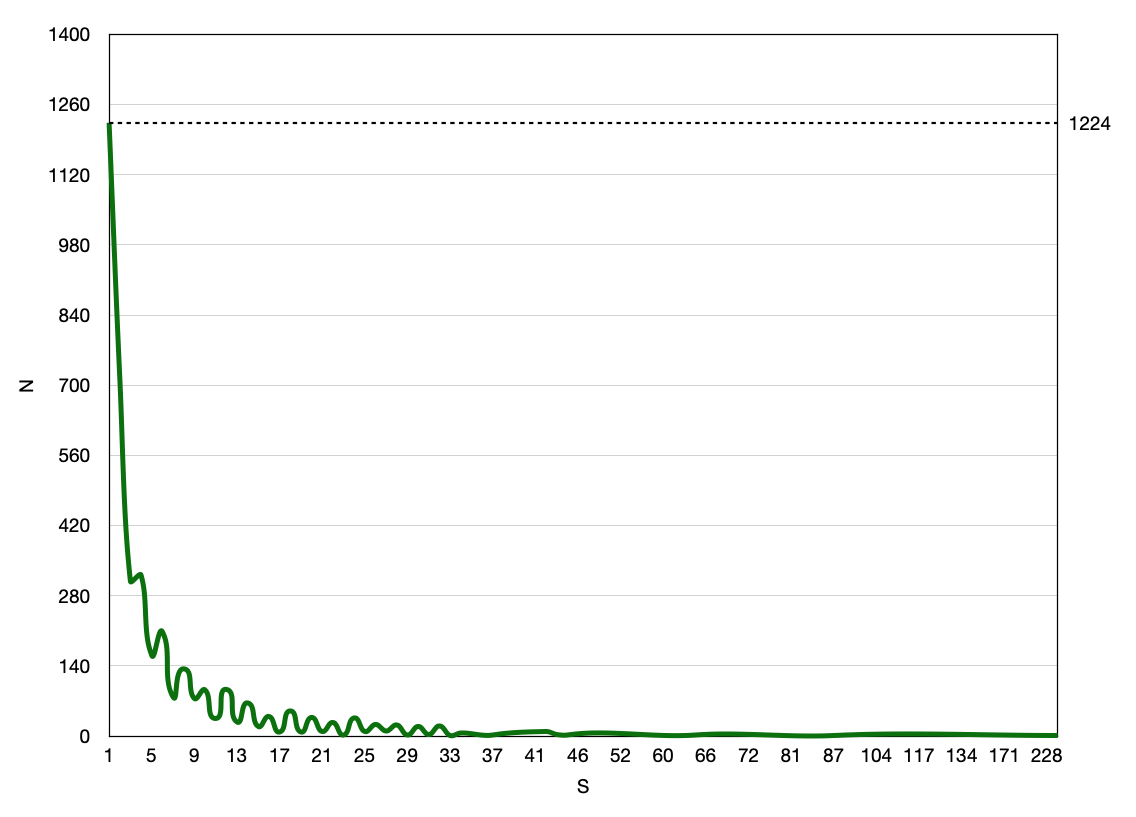
\includegraphics[width=\linewidth]{./chapter/city/Number_of_cities_having_given_number_of_sister_cities_according_to_Wikidata,_2020.png}}
}
  \caption{Зависимость числа городов всего мира (N) от числа имеющихся у этих городов побратимов (S), 2020 год.}
  \label{fig:city_relation_S_N}
\end{marginfigure}

\begin{itemize}
\item 32\% (\num{1314} городов) связаны братскими отношениями более чем с пятью городами;
\item 18\% (728 городов) имеют как минимум 11 городов-побратимов;
\item 9\% (345 городов) подружились более чем с 20 городами;
\item 2\% (94 города) имеют от 50 побратимов.
\end{itemize}

\begin{figure*}[h]
{
\setlength{\fboxsep}{0pt}%
\setlength{\fboxrule}{1pt}%
\fcolorbox{gray}{gray}{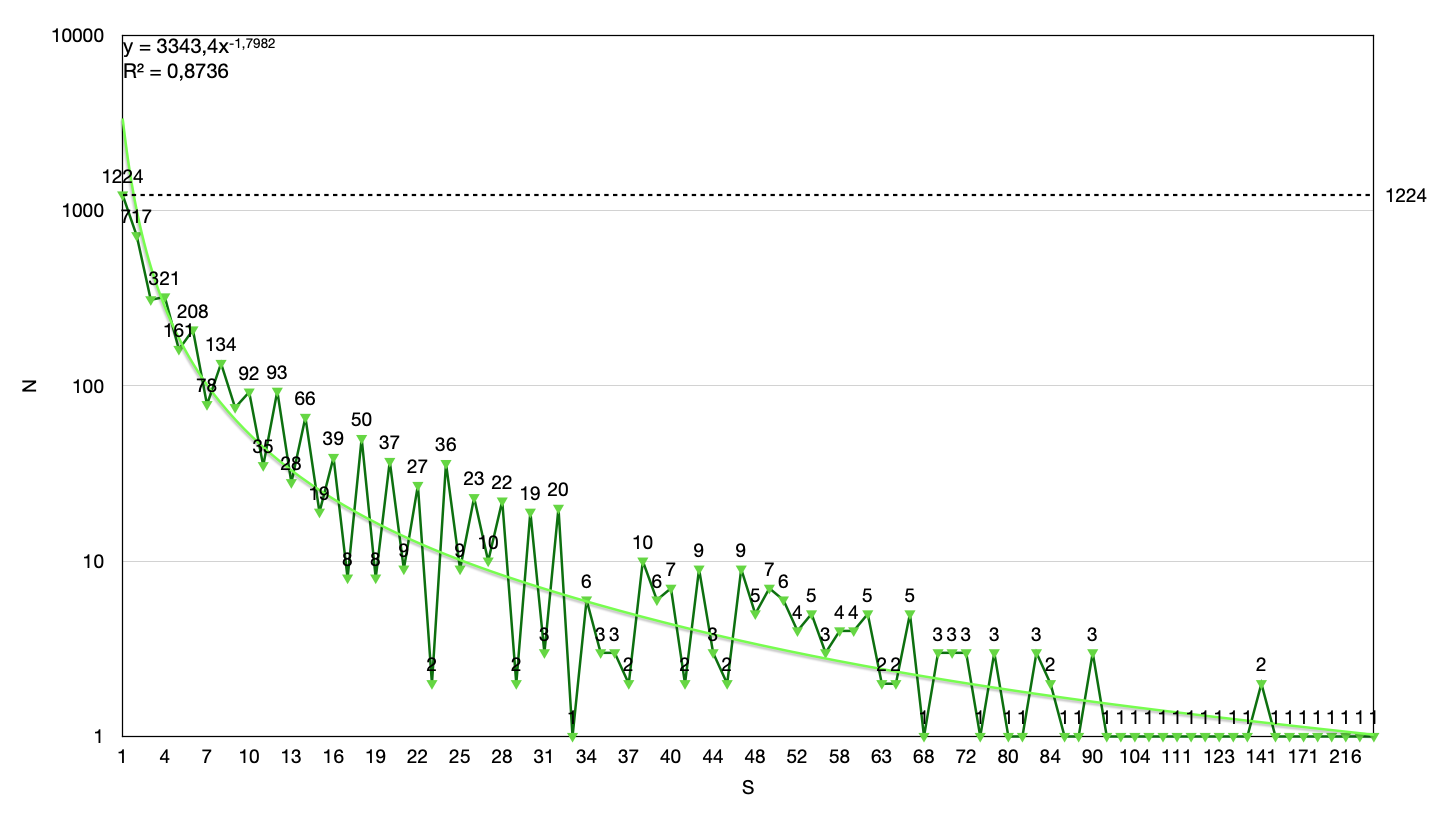
\includegraphics[width=\linewidth]{./chapter/city/Logarithm_of_the_number_of_cities_having_given_number_of_sister_cities_according_to_Wikidata,_2020.png}}%
}
  \caption{Зависимость числа городов всего мира (N) от числа имеющихся у этих городов побратимов (S) в логарифмической шкале, 2020 год.}%
  \label{fig:city_ln_relation_S_N}%
\end{figure*}

На основании построенного тренда можно сделать предположение, что зависимость числа городов от числа имеющихся у этих городов побратимов имеет распределение близкое к степенному.

\index{График!LineChart!Зависимость числа городов России (N) от числа имеющихся у этих городов побратимов (S)}
\begin{lstlisting}[ language=SPARQL, 
                    caption={\href{https://w.wiki/pMA}{Число городов России с определённым числом побратимов}\protect\footnotemark},
                    label=lst:city_relation_Russia_S_N
                    ]
#defaultView:LineChart                                                   
# Count No. of cities having sisterCount sister cities  
# and number of sister cities themselves
SELECT ?sisterCount (COUNT(?sisterCount) AS ?FreqNSister) WHERE {                                                                                  
	{ # Count sister cities of cities which are ...
		SELECT (COUNT(?sister) AS ?sisterCount) WHERE {    
			VALUES ?cityTypes {wd:Q3957 wd:Q515 wd:Q1549591 wd:Q1637706}
			?city wdt:P31 ?cityTypes. # instances of different types of cities
			?city wdt:P17 wd:Q159. # belonging to Russia
			?city wdt:P190 ?sister. # with filled property "sister city"
		}
		GROUP BY ?city # Group list by city                             
	}
}
GROUP BY ?sisterCount # Group by number of sister cities
ORDER BY DESC(?sisterCount) # Order by number of sister cities                                  
\end{lstlisting}
\footnotetext{Получено 24 варианта числа братских городов в России в 2020 году. Ссылка на SPARQL-запрос: \href{https://w.wiki/pMA}{https://w.wiki/pMA}}  

Ситуация с отечественными городами представлена на рис. \ref{fig:city_relation_Russia_S_N}. Чуть менее ста городов России (82 города) побратались хотя бы с одним городом, из них только 48\% (39 городов) связаны братскими отношениями более чем с пятью городами.

\begin{figure}
{
\setlength{\fboxsep}{0pt}%
\setlength{\fboxrule}{1pt}%
\fcolorbox{gray}{gray}{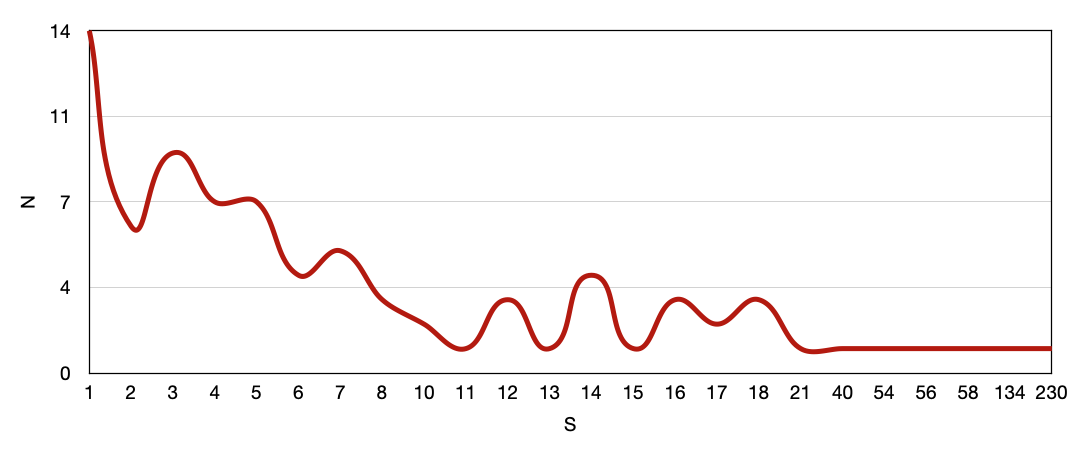
\includegraphics[width=\linewidth]{./chapter/city/Number_of_Russian_cities_having_given_number_of_sister_cities_according_to_Wikidata,_2020.png}}
}
  \caption{Зависимость числа городов России (N) от числа имеющихся у этих городов побратимов (S), 2020 год.}
  \label{fig:city_relation_Russia_S_N}
\end{figure}

\subsection{У какой страны больше всего побратимов?}

%%%%%%%%%%%%%%%% Упражнение 3 %%%%%%%%%%%%%%%%
\marginnote[-3.0cm]{
Какие из следующих городов были основаны более 400 лет назад: \href{https://w.wiki/oL8}{Москва}, \href{https://w.wiki/oL9}{Саров}, \href{https://w.wiki/oLA}{Казань}, \href{https://w.wiki/oLB}{Астрахань}, \href{https://w.wiki/oLC}{Самара}, \href{https://w.wiki/oLD}{Воронеж}?
См. ответ~\ref{answer:cities_over_400_age} на с.~\pageref{answer:cities_over_400_age}.
}

Ниже представлен SPARQL-запрос для получения списка стран, упорядоченных по числу побратимов (листинг \ref{lst:countries_sister_cities}). Результаты запроса представлены на рис. \ref{fig:Bubble_countries_sister_cities}.

\begin{marginfigure}[0.5cm]
{
\setlength{\fboxsep}{0pt}%
\setlength{\fboxrule}{1pt}%
\fcolorbox{gray}{gray}{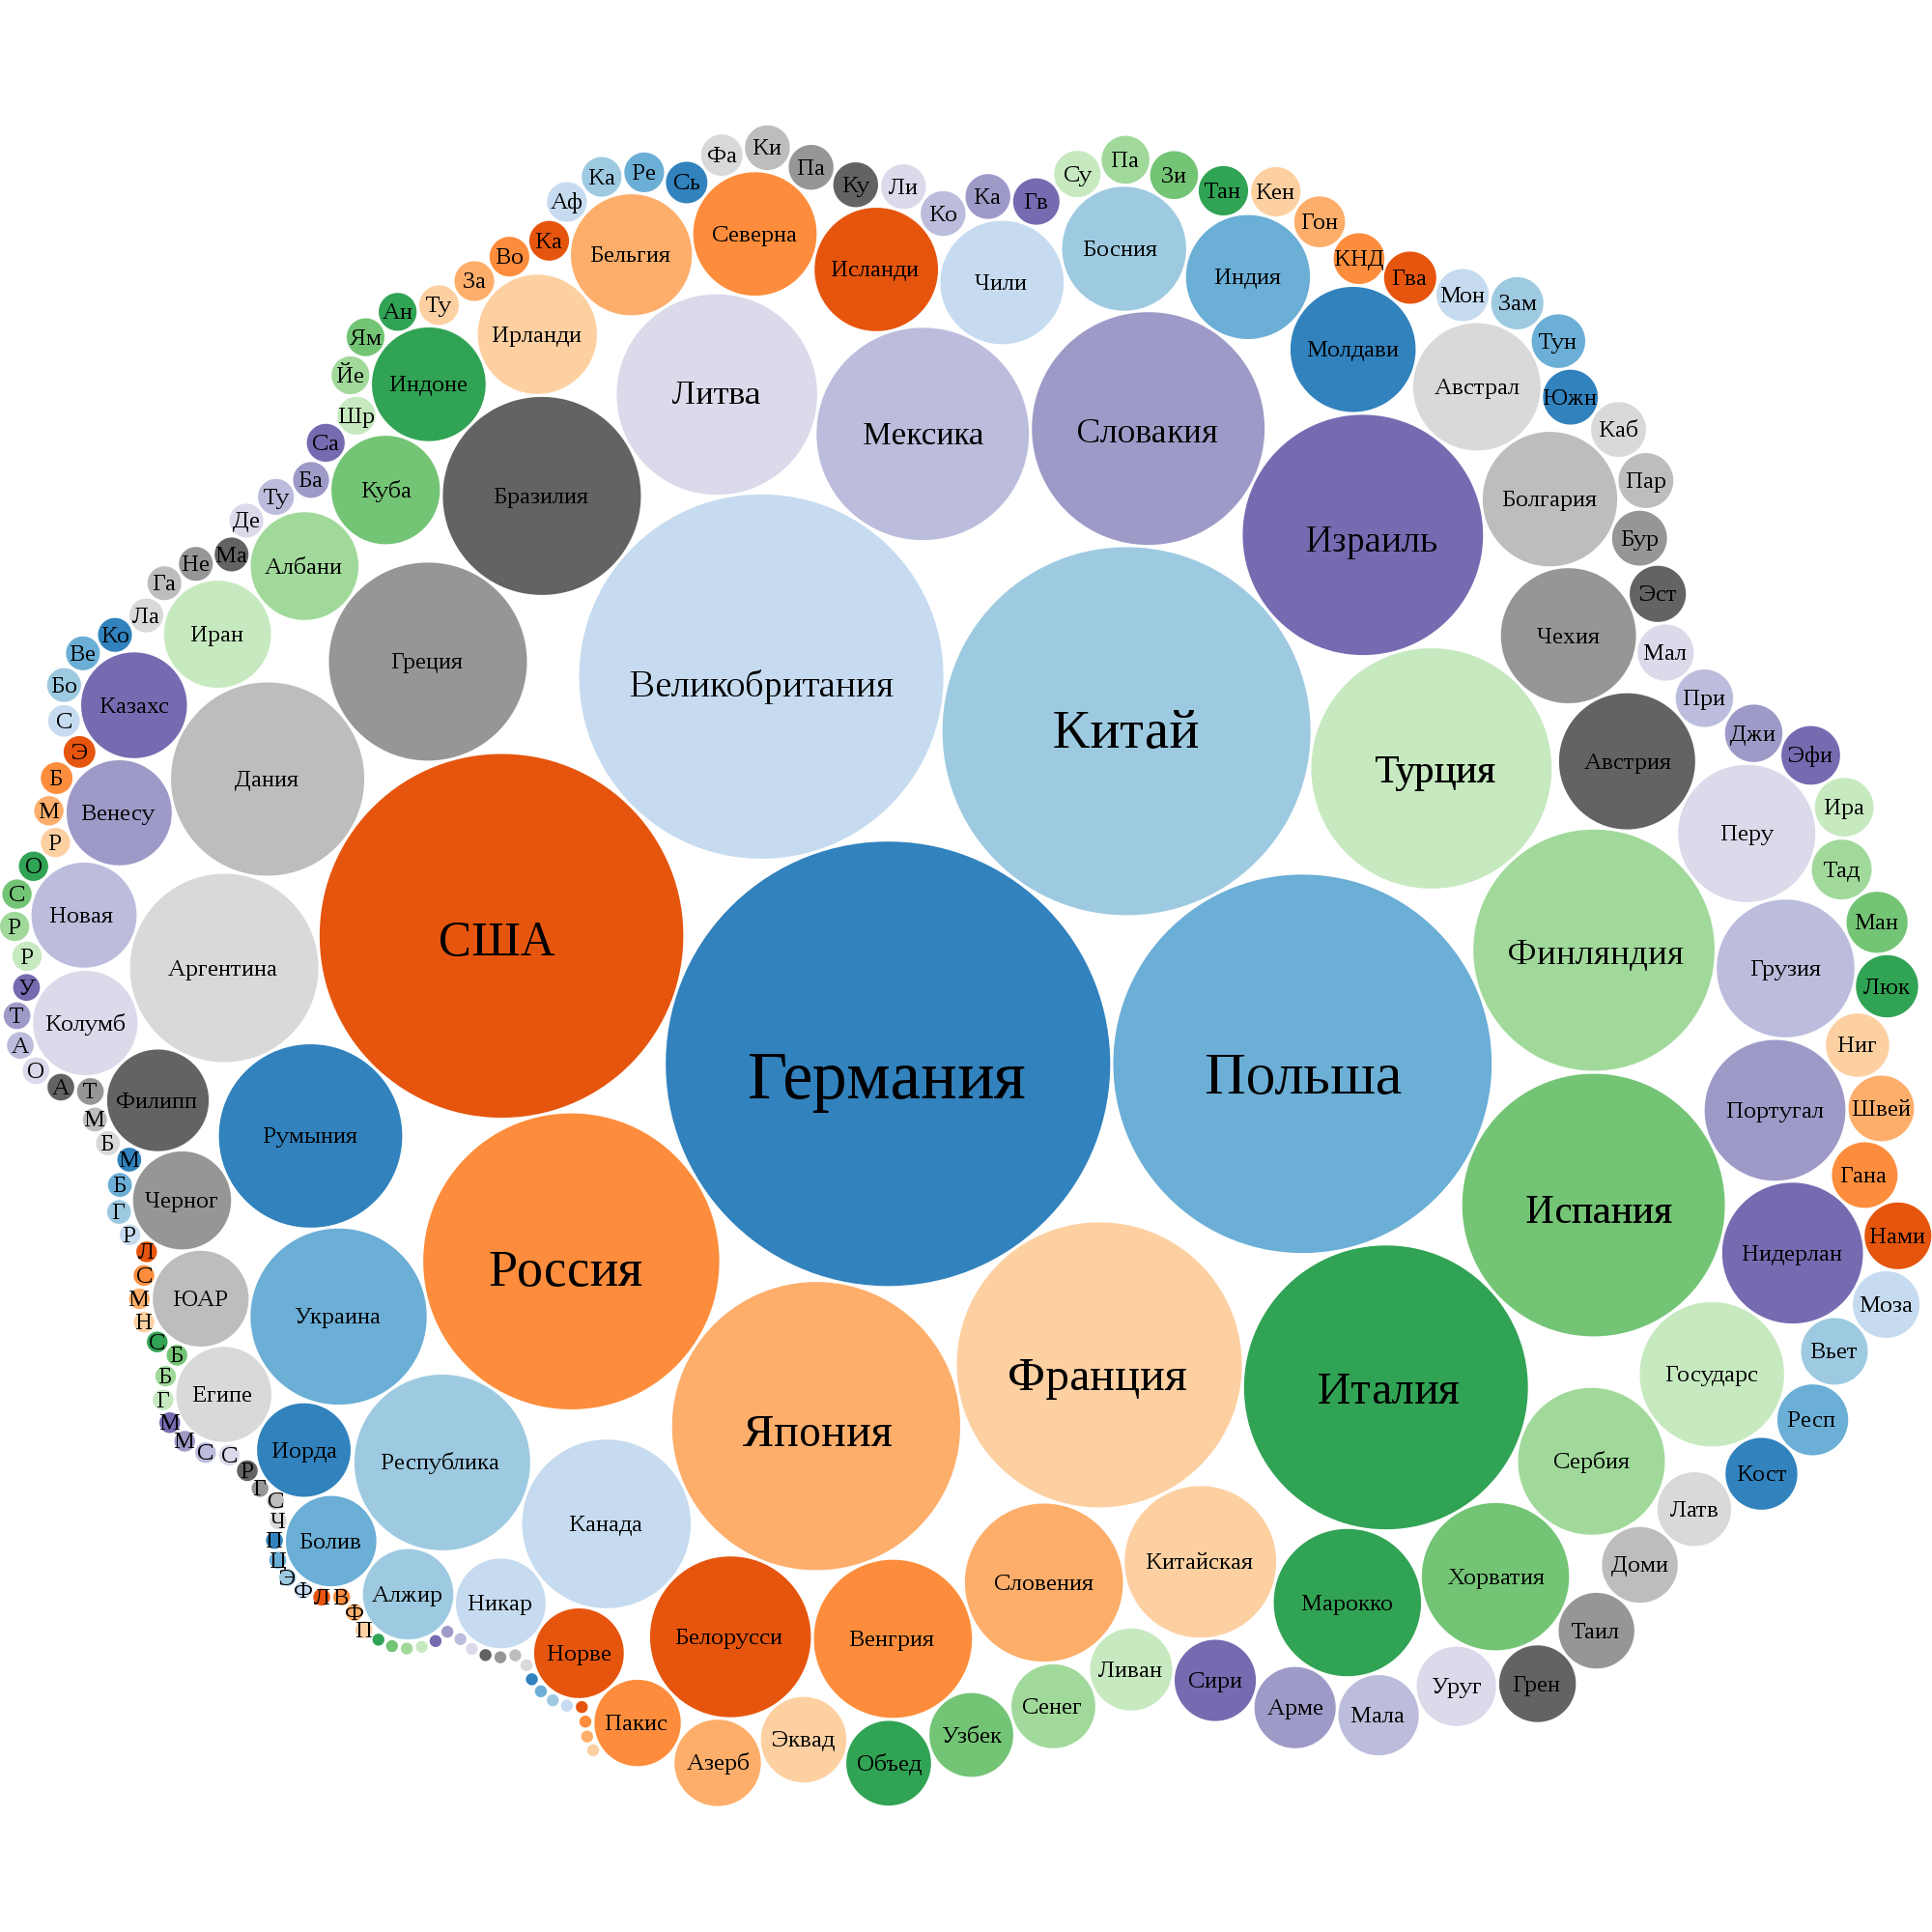
\includegraphics[width=\linewidth]{./chapter/city/Bubble_chart_number_of_sister_cities_of_countries_according_to_Wikidata,_2020_(RU).png}}%
}
  \caption[Пузырьковая диаграмма стран мира по числу побратимов у городов, 2020 год.]{Пузырьковая диаграмма стран мира, размер шарика -- число побратимов у городов страны, 2020 год.}%
  \label{fig:Bubble_countries_sister_cities}%
\end{marginfigure}

\index{SPARQL!COUNT!Упорядоченный список стран по числу побратимов}
\index{График!BubbleChart!Число побратимов у страны}
\begin{lstlisting}[ language=SPARQL, 
                    caption={\href{https://w.wiki/pMC}{Упорядоченный список стран по числу побратимов}\protect\footnotemark},
                    label=lst:countries_sister_cities
                    ]
#defaultView:BubbleChart
# Selecting number of distinct sister cities of particular country cities 
# which are ... 
SELECT ?countryLabel (COUNT(?sister) as ?sisterCount) WHERE { 
	SELECT DISTINCT ?countryLabel ?sister WHERE {
		VALUES ?cityTypes {wd:Q3957 wd:Q515 wd:Q1549591 wd:Q1637706}
		?city wdt:P31 ?cityTypes. # instances of different types of cities
		?city wdt:P17 ?country. # with filled property "country"
		?city wdt:P190 ?sister. # with filled property "sister city"
		SERVICE wikibase:label { bd:serviceParam wikibase:language "ru". }
	}                                 
}
GROUP BY ?countryLabel
ORDER BY DESC(?sisterCount)
\end{lstlisting}
\footnotetext{Получено 208 стран в 2020 году. Ссылка на SPARQL-запрос: \href{https://w.wiki/pMC}{https://w.wiki/pMC}}  

На 2020 год больше всего побратимов имела Германия (\num{1375} городов). В таблице~\ref{tab:germany_sister_cities} приведен список из 10 стран, имеющих наибольшее количество побратимов с городами Германии (2020). Получить полный список стран, с которыми Германия имеет города-побратимы, можно выполнив SPARQL-запрос, представленный ниже (листинг \ref{lst:sister_cities_with_Germany}).

\begin{table}
  \centering
  \fontfamily{ppl}\selectfont
  \begin{tabular}{| c | l | r | r |}
    \toprule
   \# & \multicolumn{1}{ c |}{Название страны} & \multicolumn{1}{p{0.3\textwidth} |}{\centering Количество городов-побратимов} & \multicolumn{1}{p{0.2\textwidth} |}{\centering \% от общего числа} \\
   \midrule
    1 & \wdqName{Франция}{142} & 247 & \num{18,0}\% \\
    2 & \wdqName{Германия}{183} & 195 & \num{14,2}\% \\
    3 & \wdqName{Великобритания}{145} & 120 & \num{8,7}\% \\
    4 & \wdqName{Италия}{38} & 86 & \num{6,3}\% \\
    5 & \wdqName{Польша}{36} & 81 & \num{5,9}\% \\
    6 & \wdqName{США}{30} & 60 & \num{4,4}\% \\
    7 & \wdqName{Австрия}{40} & 41 & \num{3,0}\% \\
    8 & \wdqName{Россия}{159} & 39 & \num{2,8}\% \\
    9 & \wdqName{Венгрия}{28} & 39 & \num{2,8}\% \\
    10 & \wdqName{Бельгия}{31} & 33 & \num{2,4}\% \\
    \bottomrule  \end{tabular}%
  \caption{Список первых 10 стран, имеющих больше всего побратимов с городами Германии на 2020 год.}
  \label{tab:germany_sister_cities}
  %\zsavepos{pos:normaltab}
\end{table}

\index{SPARQL!COUNT!Список стран, имеющих побратимов с городами Германии}
\begin{lstlisting}[ language=SPARQL, 
                    caption={\href{https://w.wiki/pME}{Список стран, имеющих побратимов с городами Германии}\protect\footnotemark},
                    label=lst:sister_cities_with_Germany
                    ]
# Selecting number of distinct particular country sister cities of cities 
# which are ...
SELECT ?country ?countryLabel 
				(COUNT(DISTINCT ?sister) as ?sisterCount) WHERE {                                                          
	VALUES ?cityTypes {wd:Q3957 wd:Q515 wd:Q1549591 wd:Q1637706}
	?city wdt:P31 ?cityTypes. # instances of different types of cities
	?city wdt:P17 wd:Q183. # belonging to Germany  
	?city wdt:P190 ?sister. # with filled property "sister city" which are
	?sister wdt:P17 ?country. # with filled property "country"
	SERVICE wikibase:label { bd:serviceParam wikibase:language "ru". }
}
GROUP BY ?country ?countryLabel
ORDER BY DESC(?sisterCount)\end{lstlisting}
\footnotetext{Получено 93 страны в 2020 году. Ссылка на SPARQL-запрос: \href{https://w.wiki/pME}{https://w.wiki/pME}} 

\subsection{Ближайшие соседи России по числу городов-побратимов}

Ниже представлен SPARQL-запрос для получения списка стран, с которыми у России есть города-побратимы (листинг \ref{lst:countries_sister_cities_with_Russia}). Результаты запроса представлены на рис. \ref{fig:Map_closest_neighbours_Russia}.

%%%%%%%%%%%%%%%% Упражнение 2 %%%%%%%%%%%%%%%%
\marginnote{
Какому городу принадлежит флаг, изображенный на рис. \ref{fig:flag_question_city}?
}

\begin{marginfigure}[0.0cm]
{
\setlength{\fboxsep}{0pt}%
\setlength{\fboxrule}{1pt}%
\fcolorbox{gray}{gray}{
\includegraphics[width=\linewidth]{./chapter/city/Flag_of_Karabulak_(Ingushetia).png}}%
}
  \caption{Флаг одного из городов России.}%
  \label{fig:flag_question_city}%
\end{marginfigure}

\marginnote{
См. ответ~\ref{answer:cities_flags} на с.~\pageref{answer:cities_flags}.
}

\index{SPARQL!COUNT!Ближайшие соседи России по числу побратимов}
\index{SPARQL!FILTER!Ближайшие соседи России по числу побратимов}
\index{SPARQL!OPTIONAL!Ближайшие соседи России по числу побратимов}
\index{SPARQL!BIND!Ближайшие соседи России по числу побратимов}
\index{SPARQL!IF!Ближайшие соседи России по числу побратимов}
\index{График!Map!Ближайшие соседи России по числу городов-побратимов}
\begin{lstlisting}[ language=SPARQL, 
                    caption={\href{https://w.wiki/q5Z}{Ближайшие соседи России по числу побратимов}\protect\footnotemark},
                    label=lst:countries_sister_cities_with_Russia
                    ]
#defaultView:Map
# Selecting number of distinct particular country sister cities of cities 
# which are ...
SELECT ?country ?countryLabel ?sisterCount ?shape ?layer WHERE {
	{ 
		SELECT ?country ?countryLabel 
						(COUNT(DISTINCT ?sister) as ?sisterCount) WHERE {  
			VALUES ?cityTypes {wd:Q3957 wd:Q515 wd:Q1549591 wd:Q1637706}
			?city wdt:P31 ?cityTypes. # instances of different types of cities
			?city wdt:P17 wd:Q159. # city belongs to Russia
			?city wdt:P190 ?sister. # city has "sister city"
			?sister wdt:P17 ?country. # which belongs to "country"
			FILTER(?country NOT IN(wd:Q159)) # except the Russia
			SERVICE wikibase:label { bd:serviceParam wikibase:language "ru". }
		}
		GROUP BY ?country ?countryLabel
		ORDER BY DESC(?sisterCount)
	}
	OPTIONAL {?country wdt:P3896 ?shape.} # country has "geoshape"
	BIND(
		IF(?sisterCount < 5, "<5",
		IF(?sisterCount <= 10, "5-10",
		IF(?sisterCount <= 20, "11-20",
		IF(?sisterCount <= 30, "21-30",
		IF(?sisterCount <= 40, "31-40",
		">40"))))) AS ?layer).
}
\end{lstlisting}
\footnotetext{Получено 102 страны в 2020 году. Ссылка на SPARQL-запрос: \href{https://w.wiki/q5Z}{https://w.wiki/q5Z}}  

\begin{figure*}[h]
{
\setlength{\fboxsep}{0pt}%
\setlength{\fboxrule}{1pt}%
\fcolorbox{gray}{gray}{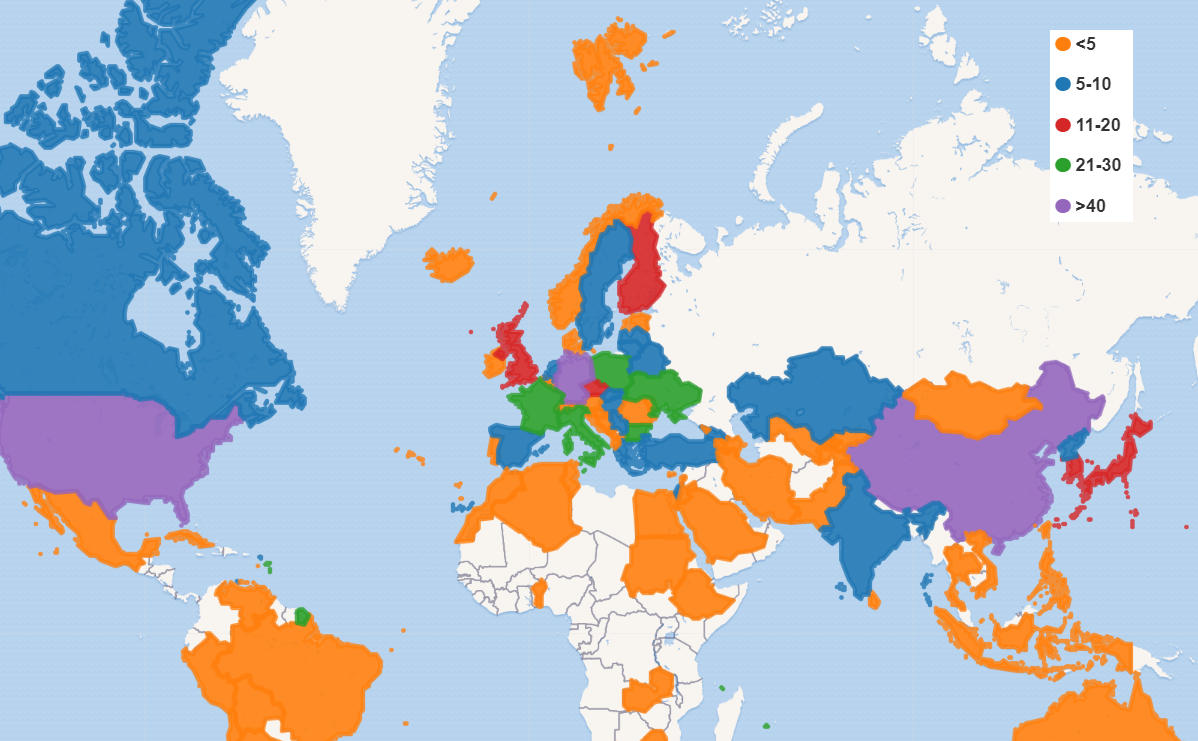
\includegraphics[width=\linewidth]{./chapter/city/Map_of_closest_neighbours_of_Russia_by_number_of_sister_cities,_2020.png}}
}
	\caption{Карта ближайших соседей России по числу городов-побратимов, 2020 год.}
	\label{fig:Map_closest_neighbours_Russia}
\end{figure*}

Больше двадцати городов-побратимов у России с такими странами, как США (46), Китай (46), Германия (44), Украина (28), Болгария (25), Польша (24), Франция (23) и Италия (22).

%%%%%%%%%%%%%%%%%%%%%%%%%%%%%%%%%%%%%%%%%%%%%%%%%%%%%%%
\section{Полнота и недостатки Викиданных}

Городом принято называть крупный населённый пункт, жители которого, как правило, не заняты сельским хозяйством. При этом разные страны используют различные критерии при наделении поселений статусом города, основным из которых является численность населения. Некоторые страны и вовсе не применяют понятие города. Так, во Франции используется только одна географическая единица подобного рода -- коммуна, вне зависимости от количества проживающих в ней людей и рода их деятельности. Поэтому чётко определить, какой населённый пункт относить к городам, а какой нет, может быть затруднительно.

На практике некоторые объекты Викиданных могут одновременно являться экземплярами городов разных типов. Например, \wdqName{Шанхай}{8686} отнесен к трём исследуемым объектам: \wdqName{city}{515}, \wdqName{big city}{1549591}, \wdqName{city with millions of inhabitants}{1637706}. Нетрудно догадаться, что такое множественное присваивание сказывается на результатах SPARQL-запросов, в частности, с использованием конструкции \href{https://en.wikibooks.org/wiki/SPARQL/UNION}{UNION}. Это несложно проверить, выполнив, например, SPARQL-запрос по нахождению городов разных типов (линстинг \ref{lst:different_city_types}). \wdqName{Шанхай}{8686} встречается в результатах три раза. 

Викиданные имеют механизм наследования, выражающийся в свойстве \href{https://www.wikidata.org/wiki/Property:P279}{subclass of}. Заключается этот механизм в том, что если объект является экземпляром \wdqName{big city}{1549591}, то он является и экземпляром  \wdqName{city}{515}, так как \wdqName{big city}{1549591} -- подкласс  \wdqName{city}{515}. Таким образом, описанную выше ситуацию с \wdqName{Шанхаем}{8686} можно разрешить, оставив только один класс \wdqName{city with millions of inhabitants}{1637706}. Стоит отметить, что замена конструкции с использованием \href{https://en.wikibooks.org/wiki/SPARQL/UNION}{UNION} (листинг \ref{lst:example_union_city}) на конструкцию с учетом подклассов неэквивалентна (листинг \ref{lst:example_subclasses_city}). Рассмотренный ранее \wdqName{Шанхай}{8686} встречается в новой выборке даже четыре раза. Дело в том, что помимо части исследуемых классов есть и другие наследуемые от \wdqName{city}{515}. Например, \wdqName{lost city}{2974842}, \wdqName{free imperial city}{57318}, \wdqName{autonomous city}{1094397} и даже \wdqName{ideal city}{1656724}.

\begin{lstlisting}[ language=SPARQL, 
                    caption={\href{https://w.wiki/k5T}{Пример использования конструкции UNION}\protect\footnotemark},
                    label=lst:example_union_city
                    ]
SELECT ?city ?cityLabel WHERE { # Selecting items which are ...
	{ ?city wdt:P31 wd:Q515 } UNION # instances of "city"            
	{ ?city wdt:P31 wd:Q1549591 } UNION # OR instances of "big city"               
	{ ?city wdt:P31 wd:Q1637706 } # OR instances of "city 1000000+"
	SERVICE wikibase:label { bd:serviceParam wikibase:language "ru". }
}
\end{lstlisting}
\footnotetext{Ссылка на SPARQL-запрос: \href{https://w.wiki/k5T}{https://w.wiki/k5T}}

\begin{lstlisting}[ language=SPARQL, 
                    caption={\href{https://w.wiki/jyB}{Пример использования конструкции с подклассами}\protect\footnotemark},
                    label=lst:example_subclasses_city
                    ]
SELECT ?city ?cityLabel WHERE { # Selecting items which are ...
	?city wdt:P31/wdt:P279* wd:Q515 # instances of "city" subclasses
	SERVICE wikibase:label { bd:serviceParam wikibase:language "ru". }
}
\end{lstlisting}
\footnotetext{Ссылка на SPARQL-запрос: \href{https://w.wiki/jyB}{https://w.wiki/jyB}}

Также, вероятно, в связи с неоднозначностью критериев присвоения статуса города, были созданы подклассы для конкретных стран -- \wdqName{city in Chile}{25412763}, \wdqName{city in Cyprus}{29556224}, \wdqName{city of Japan}{494721} и так далее. Не обошла стороной эта тенденция и города России, что можно было заметить при сравнении результатов SPARQL-запроса для нахождения экземпляров объекта <<город>> (листинг \ref{lst:city}). На 2020 год большинство из них принадлежат классу \wdqName{city/town}{7930989}.

По данным \href{https://bit.ly/2JPL34b}{всероссийской переписи населения 2010 года}\autocite{city_perepis_2010} и \href{https://bit.ly/2Lflc6F}{переписи населения в Крымском федеральном округе 2014 года}\autocite{city_perepis_2014} суммарное число городов России составило \num{1117} на 2014 год. Все \href{https://w.wiki/oLE}{города России} имеют страницу как в Русской, так и в Английской Википедии.

Число элементов Викиданных, являющихся российскими городами -- \href{https://w.wiki/jyP}{\num{1126}} . Можно предположить, что Викиданные полностью покрывают, как минимум, российские города. 

%%%%%%%%%%%%%%%%%%%%%%%%%%%%%%%%%%%%%%%%%%%%%%%%%%%%%%%
\newpage
\section{Упражнения}
\begin{enumerate}
\item Постройте граф братских городов России.
\item Получите список городов России, находящихся за полярным кругом.
\item На какой реке в России стоит наибольшее число городов?
\item У какой страны самая большая доля городов-побратимов внутри страны относительно числа побратимов, которые связывают эту страну с другими странами?
\end{enumerate}
